\documentclass[]{beamer}

\mode<presentation>
{
    % Include the theme
    \usetheme{rwth}
%    \setbeamercovered{transparent = 0}
}
\usepackage{etex}
\usepackage{microtype}
\usepackage{graphicx}
\usepackage{latexsym,amsmath,amsfonts,amssymb, mathtools, MnSymbol}
\usepackage{xspace}
\usepackage{theorem}
\usepackage{color}
\usepackage{xcolor}
\usepackage{tikz}
\usetikzlibrary{arrows,decorations.pathmorphing,positioning,fit,trees,shapes,shadows,automata,calc}
\usepackage{pgfplots}
\usepackage[numberedbib]{apacite}

\usepackage{algorithm}
\usepackage{algpseudocode}% http://ctan.org/pkg/algorithmicx
\usepackage{multirow,booktabs}
\usepackage{marvosym}
% \usepackage[
% backend=biber,
% style=alphabetic,
% citestyle=authoryear 
% ]{biblatex}
% \addbibresource{publications} %Imports bibliography file
% \nocite{*}

\DeclareMathAlphabet{\mathcal}{OMS}{cmsy}{m}{n}

%tables
\usepackage{multirow}
\usepackage{rotating}
\usepackage[clock]{ifsym}%for the clock symbol
\usepackage{rotating}
\usepackage{romannum}
\usepackage{caption}
\usepackage{cancel}
\captionsetup{labelformat=empty,labelsep=none}

%Put your commands here!

\newcommand{\sep}{\ensuremath{~\mid~}}

\newtheorem{theorem}{Theorem}[section]
\newtheorem{lemma}[theorem]{Lemma}
\newtheorem{proposition}[theorem]{Proposition}
\newtheorem{corollary}[theorem]{Corollary}
\newtheorem{definition}{Definition}[section]
\newtheorem{example}{Example}[section]
\newtheorem{question}{Question}

\newcommand{\highlight}[1]{\vspace{3 mm}{\textbf{#1}}}
\usepackage{amsmath,latexsym,amsthm,amssymb,amsfonts,amscd,stmaryrd,textcomp} % math. symbols

% Corporate design stuff
\usepackage[left=4.5cm, right=3.5cm]{geometry}
\usepackage[absolute]{textpos}
\usepackage{blindtext}
\usepackage{helvet}
\usepackage{color}





%---- language -------%
\usepackage[english]{babel} % English spelling
\usepackage[fixlanguage]{babelbib} % English literature
\selectbiblanguage{english}

% define commands with auto-spacing command \xspace
\usepackage{xspace} 
% comma placement
\usepackage{icomma} 


\usepackage[perpage]{footmisc}

\usepackage{listings}
\usepackage{float}
\usepackage{graphicx}
\usepackage{caption}
\usepackage{subcaption}

\usepackage{appendix}
\usepackage{tikz}
\usepackage{setspace}
\usepackage{xcolor}

\usepackage{enumerate}

\usepackage[plainpages=false]{hyperref}
  
\usepackage[T1]{fontenc}   


\usetikzlibrary{arrows,calc,shapes,shadows,decorations.pathmorphing,decorations.pathreplacing,automata,shapes.multipart,positioning}

\usepackage[final]{pdfpages}

\usepackage[english]{babel}
\usepackage[utf8]{inputenc}
\usepackage{algorithm}
\usepackage[noend]{algpseudocode}

\usepackage{tabularx}
\usepackage{pgfplots}
\usepackage{multirow}

\usepackage{booktabs}

\usepackage{siunitx}


\begin{document}
\RWTHtoc

\title[Incremental Linearization for SAT Modulo Real Arithmetic Solving]{Incremental Linearization for SAT Modulo Real Arithmetic Solving}

\author[Aklima Zaman]{\textcolor{RWTHblue}{Aklima Zaman}\linebreak Supervisors: Erika Ábrahám and Jürgen Giesl \linebreak Advisor: Gereon Kremer}

\institute[]{}

\date{17 April, 2019}


\frame{
	\titlepage	
}

\section{Contents}
\begin{frame}{Contents}
    \begin{itemize}
        \item \textcolor<1>{blue}{Motivation}
		\item \textcolor<2>{blue}{Incremental linearization (IL) approach}
		\begin{itemize}
		    \item \textcolor<3>{blue}{Linearization}
		\item \textcolor<4>{blue}{Example}
		\end{itemize}
		\item \textcolor<5>{blue}{Contributions}
		\begin{itemize}
		    \item \textcolor<6>{blue}{Contributions (flow chart)}
		    \item \textcolor<7>{blue}{Linearization}
		    \item \textcolor<8>{blue}{Refinement Process}
		    \item \textcolor<9>{blue}{Example}
		\end{itemize}
		\item \textcolor<10>{blue}{Experimental Results}
		\item \textcolor<11>{blue}{Future Work}
		\item \textcolor<12>{blue}{Conclusion}
    \end{itemize}
\end{frame}

\section{Motivation}
\begin{frame}{Motivation}
    \begin{itemize}
        \item \textcolor<1>{blue}{Non-linear real arithmetic (NRA) formula is hard to solve.}
		\item \textcolor<2>{blue}{Solving NRA formulas is costly in worst case.}
% 		Solving NRA formulas by Cylindrical Algebraic Decomposition (CAD) techniques requires double exponential time in worst case.
		\item \textcolor<3>{blue}{So, the applicability is restricted in practice.}
		\item \textcolor<4>{blue}{SMT techniques and tools are available for the quantifier-free linear arithmetic formula (QFLRA).}
% 		Powerful and effective SMT techniques and tools are available for the quantifier-free linear arithmetic formula (QFLRA).
		\item \textcolor<5>{blue}{Try to use LRA solving techniques for NRA.}
    \end{itemize}
\end{frame}

\section{Incremental linearization (IL) approach}
\begin{frame}{Incremental linearization (IL) approach}
% Define block styles
\tikzstyle{decision} = [diamond, draw, 
    text width=2.5em, text badly centered, node distance=3cm, inner sep=0pt]
\tikzstyle{block} = [rectangle, draw, 
    text width=12em, text centered, rounded corners, minimum height=1em]
\tikzstyle{line} = [draw, -latex']
\tikzstyle{cloud} = [draw, ellipse, node distance=3cm,
    minimum height=1em]
\begin{figure}
\centering
\scalebox{0.75}{
 \begin{tikzpicture}[node distance = 1cm, auto]
    % Place nodes\node [block] ()
    \node [block] (nra) {\textcolor<1>{blue}{NRA Formula, $\varphi$}}; 
    % \node[block, left of nra] (Phd Thesis, Ahmed Irfan, 2018)
    \node [cloud, below=0.3cm of nra] (linearization) {\textcolor<2>{blue}{Linearization}};
    \node [block, below of=linearization] (lra) {\textcolor<3>{blue}{LRA Formula, $\hat{\varphi}$}};
    \node [cloud, below=0.3cm of lra] (smtsolver) {\textcolor<4>{blue}{SMT Solver}};
    \node [block, below of=smtsolver] (satmod) {\textcolor<4>{blue}{SAT + Model $\hat{\mu}$ of $\hat{\varphi}$}};
    \node [block, right of=smtsolver, node distance=4cm, minimum height=3em, text width=7em] (unsatorunknown) {\textcolor<4>{blue}{UNSAT / UNKNOWN}};
    \node [block, below=0.3cm of satmod] (ext) {\textcolor<5>{blue}{Try to derive assignments of $\mu$ that satisfies $\varphi$}};
    \node [cloud, left=0.5cm of ext] (formula) {\textcolor<8>{blue}{$\hat{\varphi} := \hat{\varphi} \wedge \bigwedge\limits_{\psi \in A} \psi$}};
    \node [decision, below=0.3 of ext, text width=4em] (decide) {\textcolor<6>{blue}{$\mu \models \varphi ?$}};
    \node [block, right of=decide, node distance=4cm, minimum height=1em, text width=7em] (sat) {\textcolor<6>{blue}{SAT}};
    \node [block, below=0.7cm of decide] (refinement) {\textcolor<6>{blue}{Refinement for NRA}};
    \node [cloud, below=0.5cm of refinement] (setofaxioms) {\textcolor<7>{blue}{Set A of axioms unsatisfied under $\hat{\mu}$}};
    % Draw edges
    \path [line] (nra) -- (linearization);
    \path [line] (linearization) -- (lra);
    \path [line] (lra) -- (smtsolver);
    \path [line] (smtsolver) -- (satmod);
    \path [line] (smtsolver) -- (unsatorunknown);
    \path [line] (formula) |- (smtsolver);
    \path [line] (satmod) -- (ext);
    \path [line] (ext) -- (decide);
    \path [line] (decide) -- node {\textcolor<6>{blue}{No}}(refinement);
    \path [line] (decide) -- node {\textcolor<6>{blue}{Yes}}(sat);
    \path [line] (refinement) -- (setofaxioms);
    \path [line] (setofaxioms) -| (formula);
\end{tikzpicture}}
 \label{fig:system_architecture_ours}
\end{figure}
\end{frame}

\section{Linearization}
\begin{frame}{Linearization}
    $$\underbrace{ \underbrace{ \underbrace{ \underbrace{ x \ast x }\limits_{e_1 = f_{*}(x, x)} \ast \underbrace{ x \ast x }\limits_{e_1 = f_{*}(x, x)}}\limits_{e_{2} = f_{*}(e_{1}, e_{1})} \ast \underbrace{ \underbrace{ x \ast x }\limits_{e_1 = f_{*}(x, x)} \ast \underbrace{ x \ast x }\limits_{e_1 = f_{*}(x, x)}}\limits_{e_{2} = f_{*}(e_{1}, e_{1})}}\limits_{e_{3} = f_{*}(e_{2}, e_{2})} \ast x}\limits_{e_{4} = f_{*}(e_{3}, x)}$$
\end{frame}

\section{Available axiom types}
\begin{frame}{Available axiom types}
    \begin{itemize}
        \item Zero
        \item Sign
		\item Commutativity
		\item Monotonicity
		\item Tangent plane
    \end{itemize}
\end{frame}

\section{Example}
\begin{frame}{Example}
    \begin{itemize}
        \item \textcolor<1>{blue}{Input NRA formula $\varphi$ has $t_{1} \ast s_{1}$ and $t_{2} \ast s_{2}$.}
        \bigskip
        % Consider the input NRA formula $\varphi$ has the multiplication terms $t_{1} \ast s_{1}$ and $t_{2} \ast s_{2}$.
        \item \textcolor<2>{blue}{Abstraction: \quad $\underbrace{t_{1} \ast s_{1}}\limits_{f_{*}(t_{1} \ast s_{1})} \quad$ and $\quad \underbrace{t_{2} \ast s_{2}}\limits_{f_{*}(t_{2} \ast s_{2})}$}
        % $t_{1} \ast s_{1}$ and $t_{2} \ast s_{2}$ are abstracted by $f_{\ast}(t_{1}, s_{1})$ and $f_{\ast}(t_{2}, s_{2})$, respectively and an abstracted formula $\hat{\varphi}$ is being created.
		\item \textcolor<3>{blue}{Let, abstract model $\hat{\mu}$:
% 		 contains the following assignments
    $$\hat{\mu}[t_{1}] = 2, \quad \hat{\mu}[s_{1}] = 3, \quad \hat{\mu}[f_{\ast}(t_{1}, s_{1})] = 7,$$ $$\hat{\mu}[t_{2}] = 3, \quad \hat{\mu}[s_{2}] = -4, \quad \hat{\mu}[f_{\ast}(t_{2}, s_{2})] = 5$$}
    \item \textcolor<4>{blue}{These assignments violates the \textcolor<4>{green}{semantics of multiplication}.}
    \end{itemize}
    \invisible<1-4>{\textcolor<5>{blue}{\textbf{Idea:} Identify violated \textcolor{green}{LRA} properties and extend the formula with them.}}
\end{frame}

\section{Example}
\begin{frame}{Example (cont.)}
    \begin{itemize}
        \item \textcolor{red}{Abstract model $\hat{\mu}$:  $$\hat{\mu}[t_{1}] = 2, \quad \hat{\mu}[s_{1}] = 3, \quad \hat{\mu}[f_{\ast}(t_{1}, s_{1})] = 7,$$ $$\hat{\mu}[t_{2}] = 3, \quad \hat{\mu}[s_{2}] = -4, \quad \hat{\mu}[f_{\ast}(t_{2}, s_{2})] = 5$$}
        \item \textcolor<1>{blue}{Violates following tautology:
    $$((t_{2} < 0 \wedge s_{2} > 0) \vee (t_{2} > 0 \wedge s_{2} < 0)) \leftrightarrow \textcolor<2>{green}{(t_{2} \ast s_{2})} < 0$$}
        \item \textcolor<2>{blue}{Whose abstraction is:
    $$((t_{2} < 0 \wedge s_{2} > 0) \vee (t_{2} > 0 \wedge s_{2} < 0)) \leftrightarrow \textcolor<2>{green}{f_{\ast}(t_{2}, s_{2})} < 0$$}
    \end{itemize}
\end{frame}

\section{Example}
\begin{frame}{Example (cont.)}
        \begin{overlayarea}{12cm}{5.5cm}
    	\centering
    	\begin{minipage}{5cm}
    		\vspace{1cm}
    		\begin{figure}	\includegraphics<1>[scale=0.2]{../figures/phdWork_MFunc_a.pdf}
    		\end{figure}
    		\centering
    		\vspace{-0.5cm}
    		$x \ast y$
    	\end{minipage}
    	\begin{minipage}{5cm}
    		\vspace{1cm}
    		\begin{figure}	\includegraphics<1>[scale=0.2]{../figures/phdWork_MFunc_b.pdf}
    		\end{figure}
    		\centering
    		\vspace{-0.5cm}
    		$x \ast y$ (top view)
    	\end{minipage}
    \end{overlayarea}
\end{frame}

\section{Example}
\begin{frame}{Example (cont.)}
        \begin{overlayarea}{12cm}{5.5cm}
    	\centering
    	\begin{minipage}{5cm}
    		\vspace{1cm}
    		\begin{figure}	\includegraphics<1>[scale=0.2]{../figures/phdWork_MFunc_c.pdf}
    		\end{figure}
    		\centering
    		\vspace{-0.5cm}
    		$x \ast y$ and tangent plane
    	\end{minipage}
    	\begin{minipage}{5cm}
    		\vspace{1cm}
    		\begin{figure}	\includegraphics<1>[scale=0.2]{../figures/phdWork_MFunc_d.pdf}
    		\end{figure}
    		\centering
    		\vspace{-0.5cm}
    		$x \ast y$ and tangent plane (top view)
    	\end{minipage}
    \end{overlayarea}
\end{frame}

\section{Example}
\begin{frame}{Example (cont.)}
    \begin{itemize}
        \item \textcolor{red}{Abstract model $\hat{\mu}$:  $$\hat{\mu}[t_{1}] = 2, \quad \hat{\mu}[s_{1}] = 3, \quad \hat{\mu}[f_{\ast}(t_{1}, s_{1})] = 7,$$ $$\hat{\mu}[t_{2}] = 3, \quad \hat{\mu}[s_{2}] = -4, \quad \hat{\mu}[f_{\ast}(t_{2}, s_{2})] = 5$$}
        \item \textcolor<1>{blue}{Violates the Tangent-plane axiom in the points \textcolor<1>{green}{$(2, 3)$ and $(3, -4)$}}.
        \bigskip
        \item \textcolor<2-5>{blue}{At $(2, 3)$: 
\begin{table}[]
\begin{tabular}{l}
\textcolor<3>{green}{$f_{\ast}(2, s_{1}) = 2 \ast s_{1} \hspace{1mm} \wedge$}  \\
\textcolor<3>{green}{$f_{\ast}(t_{1}, 3) = 3 \ast t_{1} \hspace{1.5mm} \wedge$}  \\
\textcolor<4>{green}{$((t_{1} > 2 \wedge s_{1} < 3) \vee (t_{1} < 2 \wedge s_{1} > 3)) \rightarrow f_{\ast}(t_{1}, s_{1}) < 3 \ast t_{1} + 2 \ast s_{1} - 6 \hspace{1mm} \wedge$} \\
\textcolor<5>{green}{$((t_{1} < 2 \wedge s_{1} < 3) \vee (t_{1} > 2 \wedge s_{1} > 3)) \rightarrow f_{\ast}(t_{1}, s_{1}) > 3 \ast t_{1} + 2 \ast s_{1} - 6 \hspace{1mm} \wedge$}
\end{tabular}
\end{table}}
    \end{itemize}
\end{frame}

\section{Contributions}
\begin{frame}{Contributions}
    \begin{itemize}
        \item \textcolor<1>{blue}{This thesis adapt and improve this method.}
        \item \textcolor<2>{blue}{Linearization process is adapted by variables.}
		\item \textcolor<3>{blue}{Add 3 new axiom types for refinement.}
		\item \textcolor<4>{blue}{Experiment with different heuristics.}
    \end{itemize}
    \bigskip
    \bigskip
    \begin{itemize}
        \item \textcolor<5>{blue}{Extend abstract model $\hat{\mu}$ by guessing the assignments.}
		\item \textcolor<6>{blue}{Some refinement techniques are not implemented.}
    \end{itemize}
\end{frame}

\section{Contributions (flow chart)}
\begin{frame}{Contributions (flow chart)}

% Define block styles
\tikzstyle{decision} = [diamond, draw,
    text width=2.5em, text badly centered, node distance=3cm, inner sep=0pt]
\tikzstyle{block} = [rectangle, draw, 
    text width=12em, text centered, rounded corners, minimum height=1em]
\tikzstyle{line} = [draw, -latex']
\tikzstyle{cloud} = [draw, ellipse, node distance=3cm,
    minimum height=1em]
\begin{figure}
\centering
\scalebox{0.75}{
 \begin{tikzpicture}[node distance = 1cm, auto]
    % Place nodes\node [block] ()
    \node [block] (nra) {NRA Formula, $\varphi$};
    \node [cloud,  fill=red!20, below=0.3cm of nra] (linearization) {Linearization};
    \node [block,  below of=linearization] (lra) {LRA Formula, $\hat{\varphi}$};
    \node [cloud, below=0.3cm of lra] (smtsolver) {SMT Solver};
    \node [block, below of=smtsolver] (satmod) {SAT + Model $\hat{\mu}$ of $\hat{\varphi}$};
    \node [block, right of=smtsolver, node distance=4cm, minimum height=3em, text width=7em] (unsatorunknown) {UNSAT / UNKNOWN};
    \node [block,  fill=red!20, below=0.3cm of satmod] (ext) {Extend $\hat{\mu}$ to assign all variables in  $\varphi$};
    \node [cloud, left=0.5cm of ext] (formula) {$\hat{\varphi} := \hat{\varphi} \wedge \bigwedge\limits_{\psi \in A} \psi$};
    \node [decision, below=0.3 of ext, text width=4em] (decide) {$\mu \models \varphi ?$};
    \node [block, right of=decide, node distance=4cm, minimum height=1em, text width=7em] (sat) {SAT};
    \node [block,  fill=red!20, below=0.7cm of decide] (refinement) {Refinement for NRA};
    \node [cloud, below=0.5cm of refinement] (setofaxioms) {Set A of axioms unsatisfied under $\hat{\mu}$};
    % Draw edges
    \path [line] (nra) -- (linearization);
    \path [line] (linearization) -- (lra);
    \path [line] (lra) -- (smtsolver);
    \path [line] (smtsolver) -- (satmod);
    \path [line] (smtsolver) -- (unsatorunknown);
    \path [line] (formula) |- (smtsolver);
    \path [line] (satmod) -- (ext);
    \path [line] (ext) -- (decide);
    \path [line] (decide) -- node {No}(refinement);
    \path [line] (decide) -- node {Yes}(sat);
    \path [line] (refinement) -- (setofaxioms);
    \path [line] (setofaxioms) -| (formula);
\end{tikzpicture}}
 \label{fig:system_architecture_ours}
\end{figure}
\end{frame}

\section{Linearization}
\begin{frame}{Linearization}
    \begin{itemize}
        \item {$$\underbrace{ \underbrace{ \underbrace{ \underbrace{ x \ast x }\limits_{e_1 = f_{*}(x, x)} \ast \underbrace{ x \ast x }\limits_{e_1 = f_{*}(x, x)}}\limits_{e_{2} = f_{*}(e_{1}, e_{1})} \ast \underbrace{ \underbrace{ x \ast x }\limits_{e_1 = f_{*}(x, x)} \ast \underbrace{ x \ast x }\limits_{e_1 = f_{*}(x, x)}}\limits_{e_{2} = f_{*}(e_{1}, e_{1})}}\limits_{e_{3} = f_{*}(e_{2}, e_{2})} \ast x}\limits_{e_{4} = f_{*}(e_{3}, x)}$$}
        \item \textcolor{blue}{$$\underbrace{ \underbrace{ \underbrace{ \underbrace{ x \ast x }\limits_{z_{1}} \ast \underbrace{ x \ast x }\limits_{z_{1}}}\limits_{z_{2}} \ast \underbrace{ \underbrace{ x \ast x }\limits_{z_{1}} \ast \underbrace{ x \ast x }\limits_{z_{1}}}\limits_{z_{2}}}\limits_{z_{3}} \ast x}\limits_{z_{4}}$$}
    \end{itemize}
\end{frame}

\section{Refinement Process}
\begin{frame}{Refinement Process}
    \textcolor<1>{blue}{\textbf{Available axiom types: }Zero, \textcolor<3>{green}{Sign, Commutativity}, Monotonicity, Tangent plane.}
    \bigskip
    \bigskip
    \begin{itemize}
        \item \textcolor<2-4>{blue}{Removed axioms:}
            \begin{itemize}
                \item \textcolor<3>{blue}{Sign}
                \item \textcolor<3>{blue}{Commutativity}
                \item \textcolor<4>{blue}{Concave solution sets}
            \end{itemize}
        \bigskip
        \bigskip
        \item \textcolor<5>{blue}{Added axioms:}
            \begin{itemize}
                \item \textcolor<5>{blue}{Square expression $z = x^2$}
                \item \textcolor<5>{blue}{Congruence for multiplications}
                \item \textcolor<5>{blue}{Integral constraint propagation (ICP)}
            \end{itemize}
    \end{itemize}
\end{frame}

\section{Refinement Process}
\begin{frame}{Refinement Process (Cont.)}
    \textbf{ICP (two dimensional case)}
    \bigskip
    \bigskip
   \begin{itemize}
   \item \textcolor<1>{blue}{Consider, \textcolor<1>{green}{$z = x*y$}.}
   \item \textcolor<2>{blue}{Absolute values of $x, y \text{ and } z$:
\textcolor<2>{green}{$$|\mu(x)| = a, \quad  |\mu(y)| = b \quad \text{ and } \quad |\mu(z)| = c$$}}
\end{itemize}
\end{frame}

\section{Refinement Process}
\begin{frame}{Refinement Process (Cont.)}
    \textbf{ICP (two dimensional case)}\newline
    
    \textcolor{red}{If the product $c$ is assumed too low ($c < a \ast b$):}
    \begin{overlayarea}{12cm}{5.5cm}
    	\centering
    	\begin{minipage}{5cm}
    		\vspace{1cm}
    		\begin{figure}	\includegraphics<1>[scale=0.8]{../figures/ICP1_1.pdf}
    		\end{figure}
    		\centering
    		\vspace{-0.5cm}
    		Choose, $\frac{c}{a} < b^\prime \leq b$
    	\end{minipage}
    	\begin{minipage}{5cm}
    		\vspace{1cm}
    		\begin{figure}	\includegraphics<1>[scale=0.8]{../figures/ICP1_2.pdf}
    		\end{figure}
    		\centering
    		\vspace{-0.5cm}
    		Choose, $\frac{c}{b^\prime} < a^\prime \leq a$
    	\end{minipage}
    \end{overlayarea}
\end{frame}

\section{Refinement Process}
\begin{frame}{Refinement Process (Cont.)}
    \textbf{ICP (two dimensional case)}\newline
    
    So, for \textcolor{green}{$c < a \ast b$} we have two axioms:
    \bigskip
    \bigskip
    \begin{itemize}
        \item \textcolor{blue}{$$((x \geq a^\prime \wedge y \geq b^\prime) \vee (x \leq -a^\prime \wedge y \leq -b^\prime)) \rightarrow (z \geq c^\prime)$$}
        \item \textcolor{blue}{$$((x \geq a^\prime \wedge y \leq -b^\prime) \vee (x \leq -a^\prime \wedge y \geq b^\prime)) \rightarrow (z \leq -c^\prime)$$}
    \end{itemize}
\end{frame}

% \section{Refinement Process}
% \begin{frame}{Refinement Process (Cont.)}
%     \textbf{ICP (two dimensional case)}\newline If the product $c$ is assumed too high ($c > a \ast b$):
%     \begin{overlayarea}{12cm}{5.5cm}
%     	\centering
%     	\begin{minipage}{5cm}
%     		\vspace{1cm}
%     		\begin{figure}	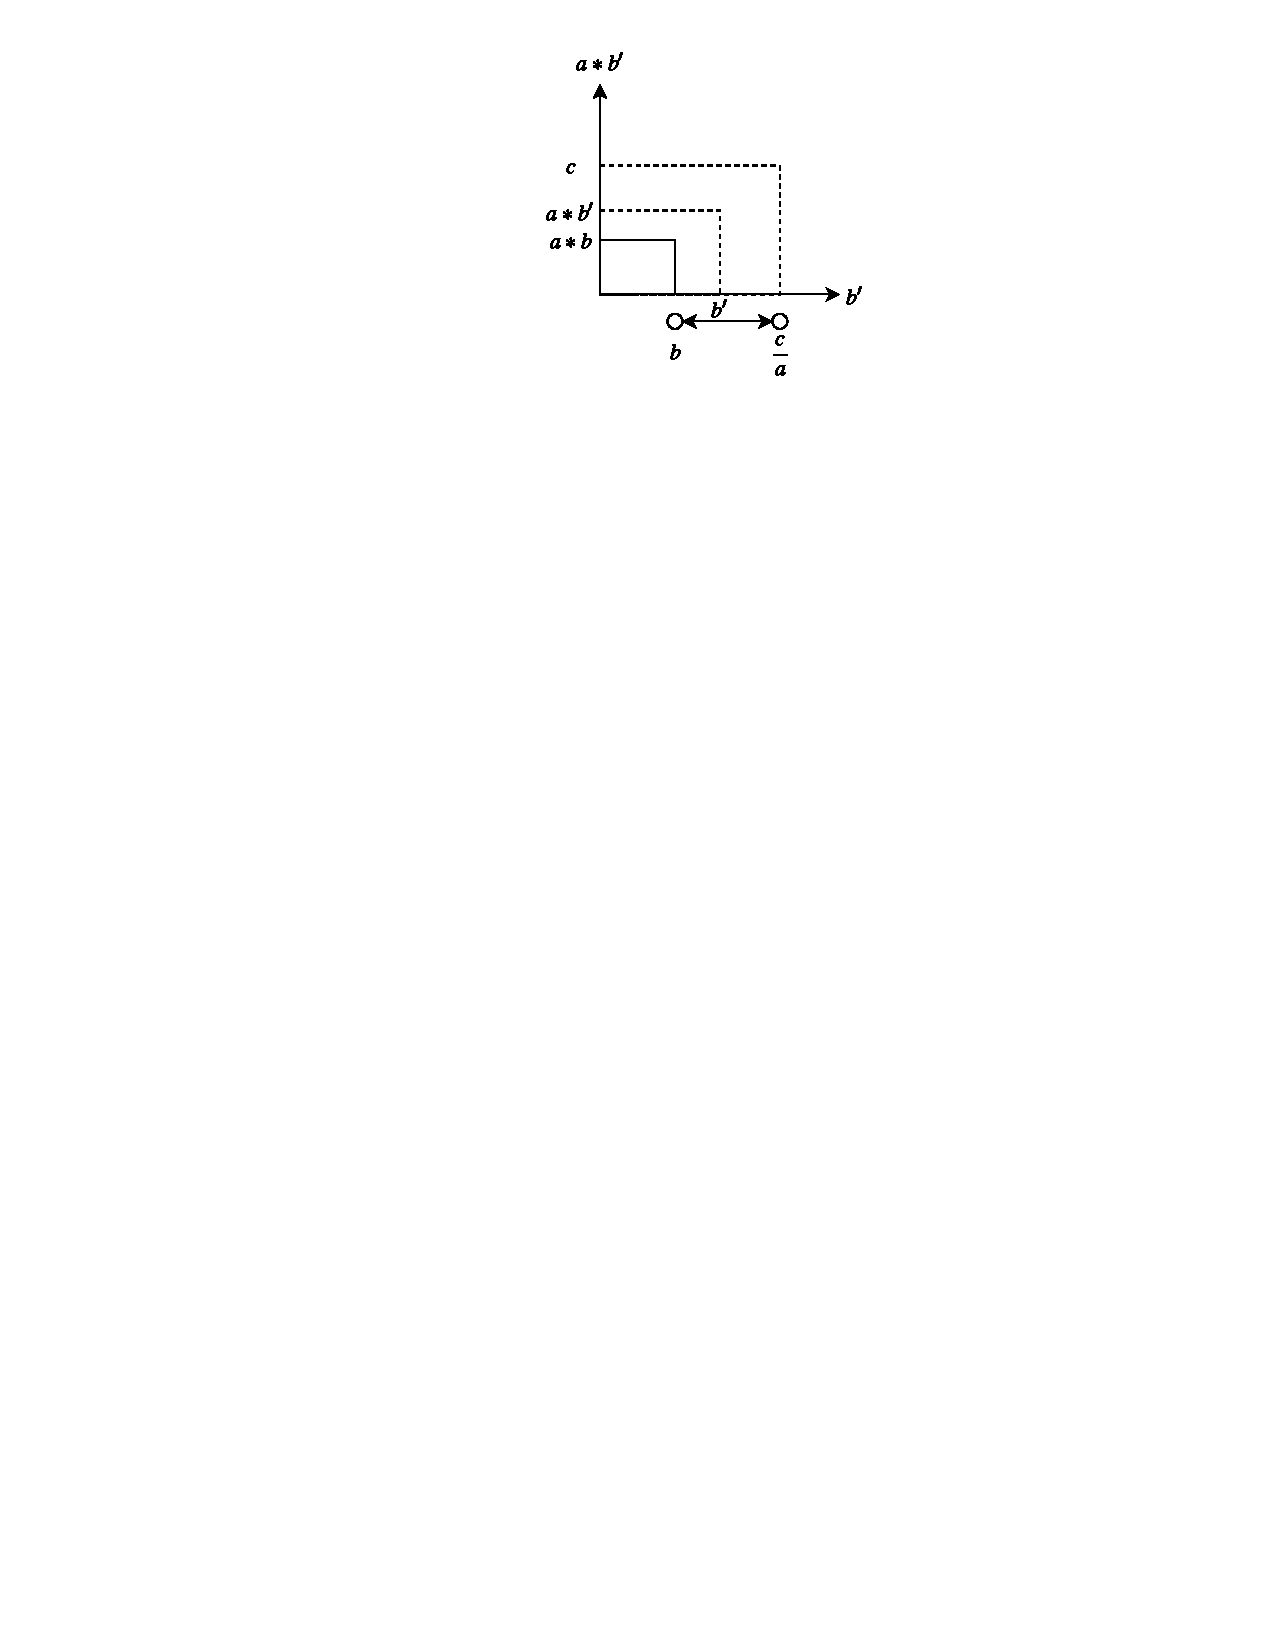
\includegraphics[scale=0.8]{../figures/ICP2_1.pdf}
%     		\end{figure}
%     		\centering
%     		\vspace{-0.5cm}
%     		Choose, $b \leq b^\prime < \frac{c}{a}$
%     	\end{minipage}
%     	\begin{minipage}{5cm}
%     		\vspace{1cm}
%     		\begin{figure}	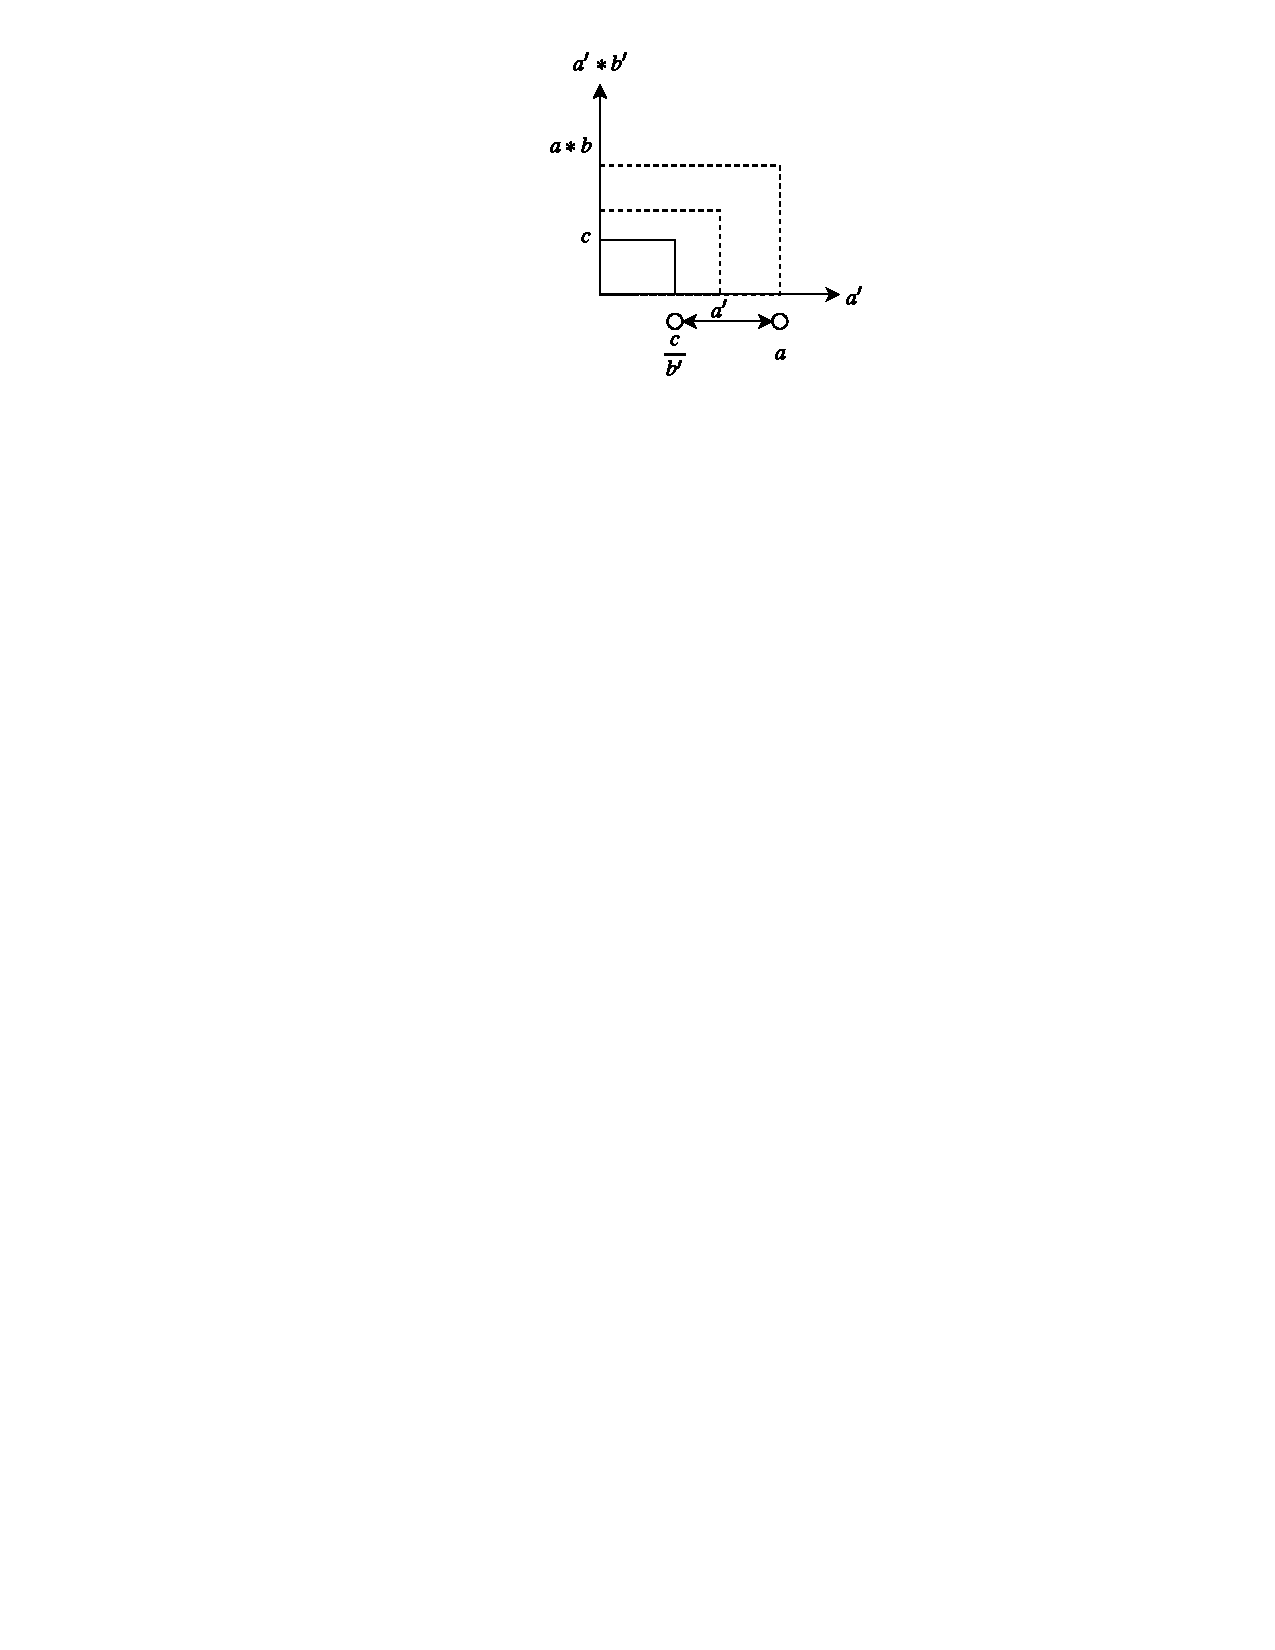
\includegraphics[scale=0.8]{../figures/ICP2_2.pdf}
%     		\end{figure}
%     		\centering
%     		\vspace{-0.5cm}
%     		Choose, $a \leq a^\prime < \frac{c}{b^\prime}$
%     	\end{minipage}
%     \end{overlayarea}
% \end{frame}

\section{Refinement Process}
\begin{frame}{Refinement Process (Cont.)}
     \textbf{ICP (two dimensional case)}\newline 
     
     \textcolor{red}{If the product $c$ is assumed too high \textcolor{green}{($c > a \ast b$):}}
     \bigskip
     \bigskip
    \textcolor{blue}{$$(-a^\prime \leq x \leq a^\prime) \wedge (-b^\prime \leq y \leq b^\prime) \rightarrow (-c^\prime \leq z \leq c^\prime)$$}
\end{frame}

\section{Refinement Process}
\begin{frame}{Refinement Process (Cont.)}
    \textbf{ICP (one dimensional case)}
    \bigskip
    \bigskip
   \begin{itemize}
   \item \textcolor<1>{blue}{Consider, \textcolor<1>{green}{$z = x*y$}.}
   \item \textcolor<2>{blue}{Absolute values of $x, \text{ and } z$:
\textcolor<2>{green}{$$|\mu(x)| = a, \quad  \text{ and } \quad |\mu(z)| = c$$}}
\end{itemize}
\end{frame}

\section{Example}
\begin{frame}{Example}
    \begin{itemize}
        \item \textcolor<1>{blue}{Input NRA formula $\varphi$ has $t_{1} \ast s_{1}$ and $t_{2} \ast s_{2}$.}
        \bigskip
        % Consider the input NRA formula $\varphi$ has the multiplication terms $t_{1} \ast s_{1}$ and $t_{2} \ast s_{2}$.
        \item \textcolor<2>{blue}{Abstraction: \quad $\underbrace{t_{1} \ast s_{1}}\limits_{z_{1}} \quad$ and $\quad \underbrace{t_{2} \ast s_{2}}\limits_{z_{2}}$}
        % $t_{1} \ast s_{1}$ and $t_{2} \ast s_{2}$ are abstracted by $f_{\ast}(t_{1}, s_{1})$ and $f_{\ast}(t_{2}, s_{2})$, respectively and an abstracted formula $\hat{\varphi}$ is being created.
		\item \textcolor<3>{blue}{Assume, abstract model $\hat{\mu}$:
% 		 contains the following assignments
    $$\hat{\mu}[t_{1}] = 2, \quad \hat{\mu}[s_{1}] = 3, \quad \hat{\mu}[f_{\ast}(t_{1}, s_{1})] = 7,$$ $$\hat{\mu}[t_{2}] = 3, \quad \hat{\mu}[s_{2}] = -4, \quad \hat{\mu}[f_{\ast}(t_{2}, s_{2})] = 5$$}
    \end{itemize}
\end{frame}

\section{Example}
\begin{frame}{Example (cont.)}
    \begin{itemize}
        \item \textcolor{red}{Abstract model $\hat{\mu}$:  $$\hat{\mu}[t_{1}] = 2, \quad \hat{\mu}[s_{1}] = 3, \quad \hat{\mu}[f_{\ast}(t_{1}, s_{1})] = 7,$$ $$\hat{\mu}[t_{2}] = 3, \quad \hat{\mu}[s_{2}] = -4, \quad \hat{\mu}[f_{\ast}(t_{2}, s_{2})] = 5$$}
        \item \textcolor<1>{blue}{Violates following  Zero tautology:
    $$((t_{2} < 0 \wedge s_{2} > 0) \vee (t_{2} > 0 \wedge s_{2} < 0)) \leftrightarrow \textcolor<2>{green}{(t_{2} \ast s_{2})} < 0$$}
        \item \textcolor<2>{blue}{Whose abstraction was:
    $$((t_{2} < 0 \wedge s_{2} > 0) \vee (t_{2} > 0 \wedge s_{2} < 0)) \leftrightarrow \textcolor<2>{green}{f_{\ast}(t_{2}, s_{2})} < 0$$}
        \item \textcolor<2>{blue}{Now, abstraction is:
    $$((t_{2} < 0 \wedge s_{2} > 0) \vee (t_{2} > 0 \wedge s_{2} < 0)) \leftrightarrow \textcolor<2>{green}{z_{2}} < 0$$}
    \end{itemize}
\end{frame}

\section{Example}
\begin{frame}{Example (cont.)}
    \begin{itemize}
        \item \textcolor{red}{Abstract model $\hat{\mu}$:  $$\hat{\mu}[t_{1}] = 2, \quad \hat{\mu}[s_{1}] = 3, \quad \hat{\mu}[f_{\ast}(t_{1}, s_{1})] = 7,$$ $$\hat{\mu}[t_{2}] = 3, \quad \hat{\mu}[s_{2}] = -4, \quad \hat{\mu}[f_{\ast}(t_{2}, s_{2})] = 5$$}
        \item \textcolor<1>{blue}{Violates the Tangent-plane axiom in the points \textcolor<1>{green}{$(2, 3)$ and $(3, -4)$}}.
        \item \textcolor<2>{blue}{At $(2, 3)$: 
\begin{table}[]
\begin{tabular}{l}
$f_{\ast}(2, s_{1}) = 2 \ast s_{1} \hspace{1mm} \wedge$  \\
$f_{\ast}(t_{1}, 3) = 3 \ast t_{1} \hspace{1.5mm} \wedge$ \\
$((t_{1} > 2 \wedge s_{1} < 3) \vee (t_{1} < 2 \wedge s_{1} > 3)) \rightarrow \textcolor<2>{green}{z_{1}} < 3 \ast t_{1} + 2 \ast s_{1} - 6 \hspace{1mm} \wedge$ \\
$((t_{1} < 2 \wedge s_{1} < 3) \vee (t_{1} > 2 \wedge s_{1} > 3)) \rightarrow \textcolor<2>{green}{z_{1}} > 3 \ast t_{1} + 2 \ast s_{1} - 6 \hspace{1mm} \wedge$
\end{tabular}
\end{table}}
    \end{itemize}
\end{frame}

\section{Experimental Results}
\begin{frame}{Experimental Results}
    \begin{itemize}
        \item \textcolor<1>{blue}{We have 7 \textcolor<1>{green}{sequences} of axioms, i.e., Zero, Tangent plane, ICP, Congruence, Monotonicity.} 
        \bigskip
        \bigskip
        \item \textcolor<2-5>{blue}{Heuristics}
        \bigskip
        \begin{itemize}
            \item \textcolor<3>{blue}{Take the \textcolor<3>{green}{first} axiom instance that is violated by the solution for the abstraction.}
            \bigskip
            \item \textcolor<4>{blue}{Take \textcolor<4>{green}{all} violated axiom instances.}
            \bigskip
            \item \textcolor<5>{blue}{Choose axiom instances \textcolor<5>{green}{randomly} from the set of all violated axiom instances.}
        \end{itemize}
    \end{itemize}
\end{frame}

\section{Experimental Results}
\begin{frame}{Experimental Results}
\textbf{SMT-RAT}
\bigskip
\bigskip
\begin{itemize}
    \item \textcolor<1>{blue}{An open source toolbox for SMT solving.}
    \bigskip
    \item \textcolor<2>{blue}{A collection of SMT compliant implementations of methods.}
    \bigskip
    \item  \textcolor<3>{blue}{Solves quantifier-free LRA, NRA, LIA, NIA formulas.}
    \bigskip
    \item \textcolor<4>{blue}{Modules are the elementary architectural component.}
\end{itemize}
\bigskip
\invisible<1-4>{\textcolor<5>{blue}{\textbf{SMT-RAT IL solvers:} \hspace{1mm} smtrat(\hspace{1mm}heuristic no.,\hspace{1mm} sequence no.)}}
\end{frame}

\section{Experimental Results}
\begin{frame}{Experimental Results}
\begin{figure}
    \caption{Number of solved instances for SMT-RAT solvers without preprocessing (WoP)}
    \centering
    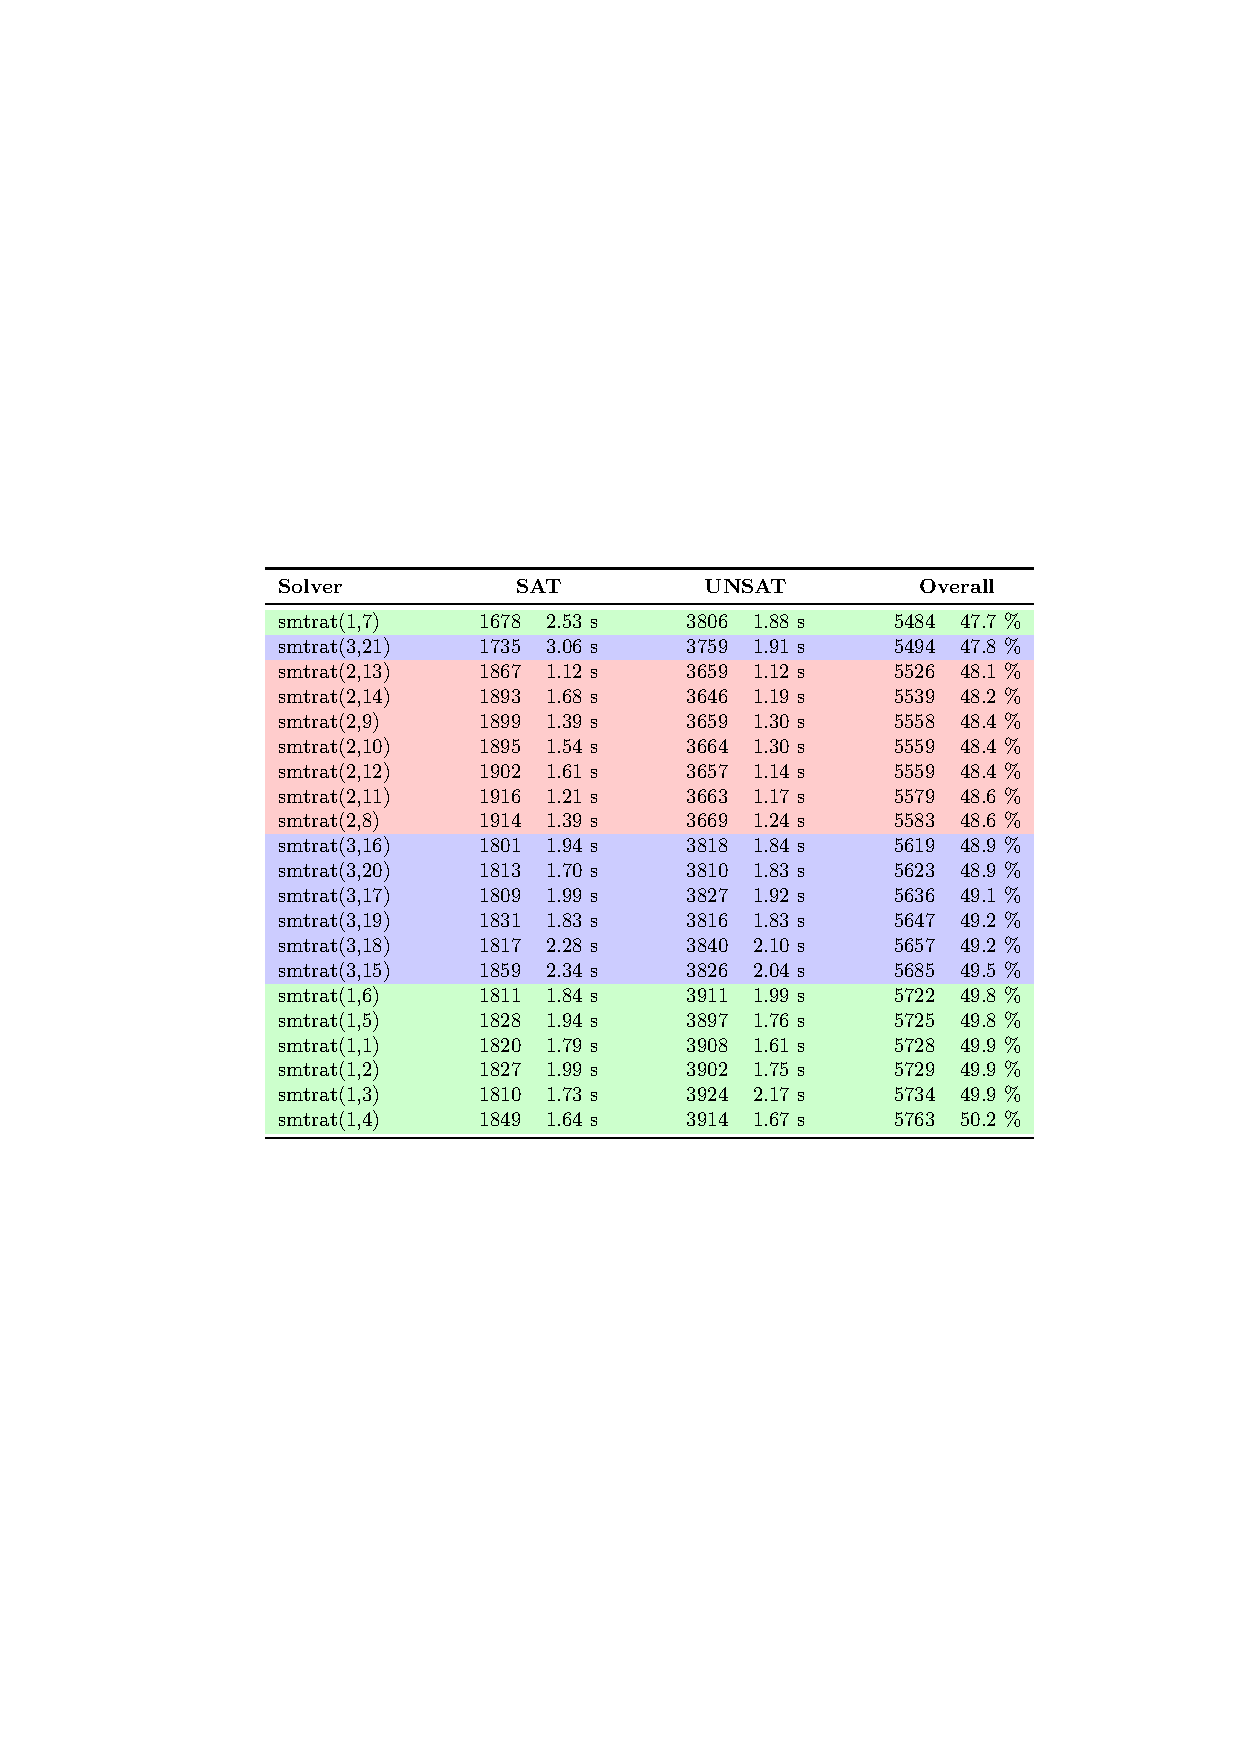
\includegraphics[scale=0.7]{../figures/OurSolver.pdf}
\end{figure}
\end{frame}

\section{Experimental Results}
\begin{frame}{Experimental Results}
\begin{figure}
    \caption{Comparison of smtrat(1, 4) with MathSAT and Z3}
    \centering
    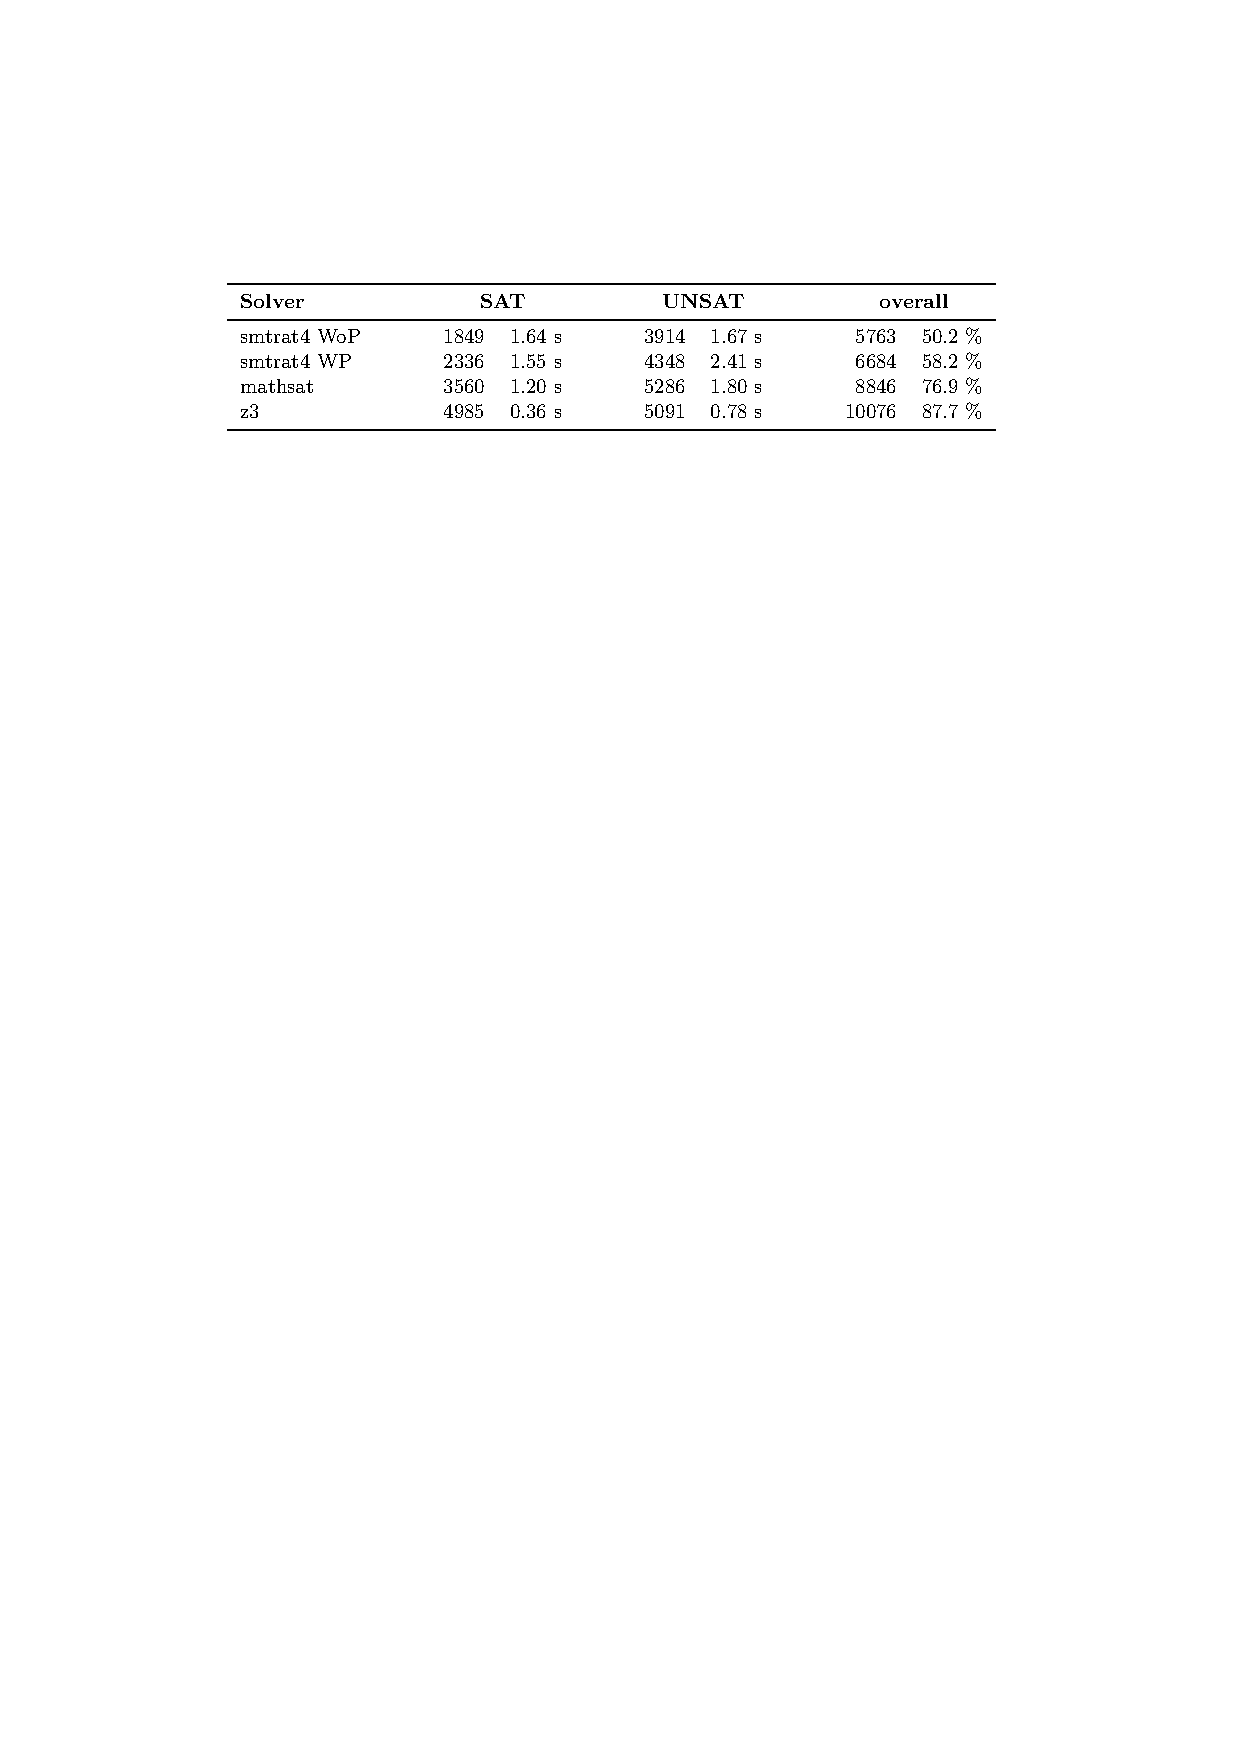
\includegraphics[scale=0.9]{../figures/ComparisonWithOthers.pdf}
\end{figure}
\end{frame}

\section{Experimental Results}
\begin{frame}{Experimental Results}
\begin{figure}
    \caption{Survival plots}
    \centering
    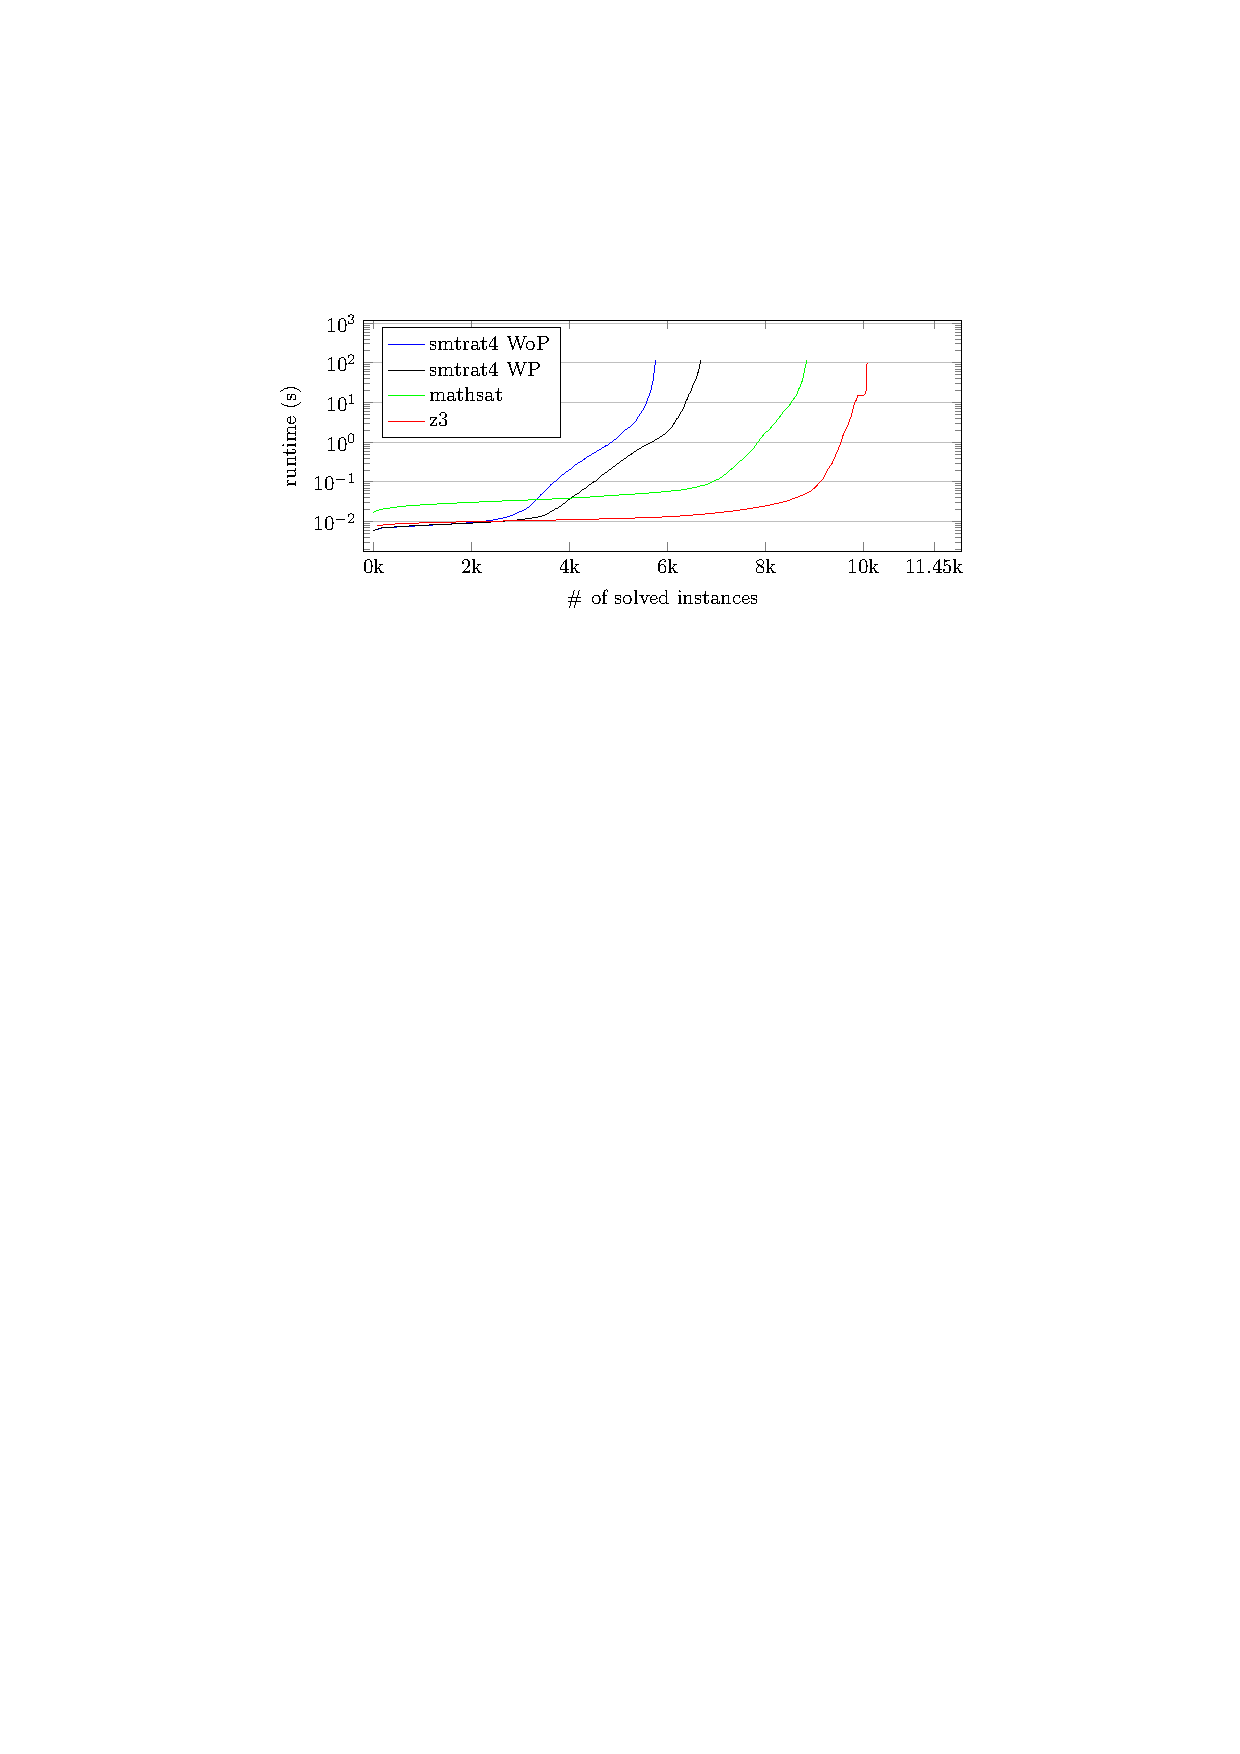
\includegraphics[scale=1]{../figures/solved_instances.pdf}
\end{figure}
\end{frame}

\section{Experimental Results}
\begin{frame}{Experimental Results}
\begin{figure}[!ht]
    \centering
    \caption{Scatter plot for smtrat(1, 4) WP and MathSAT}
    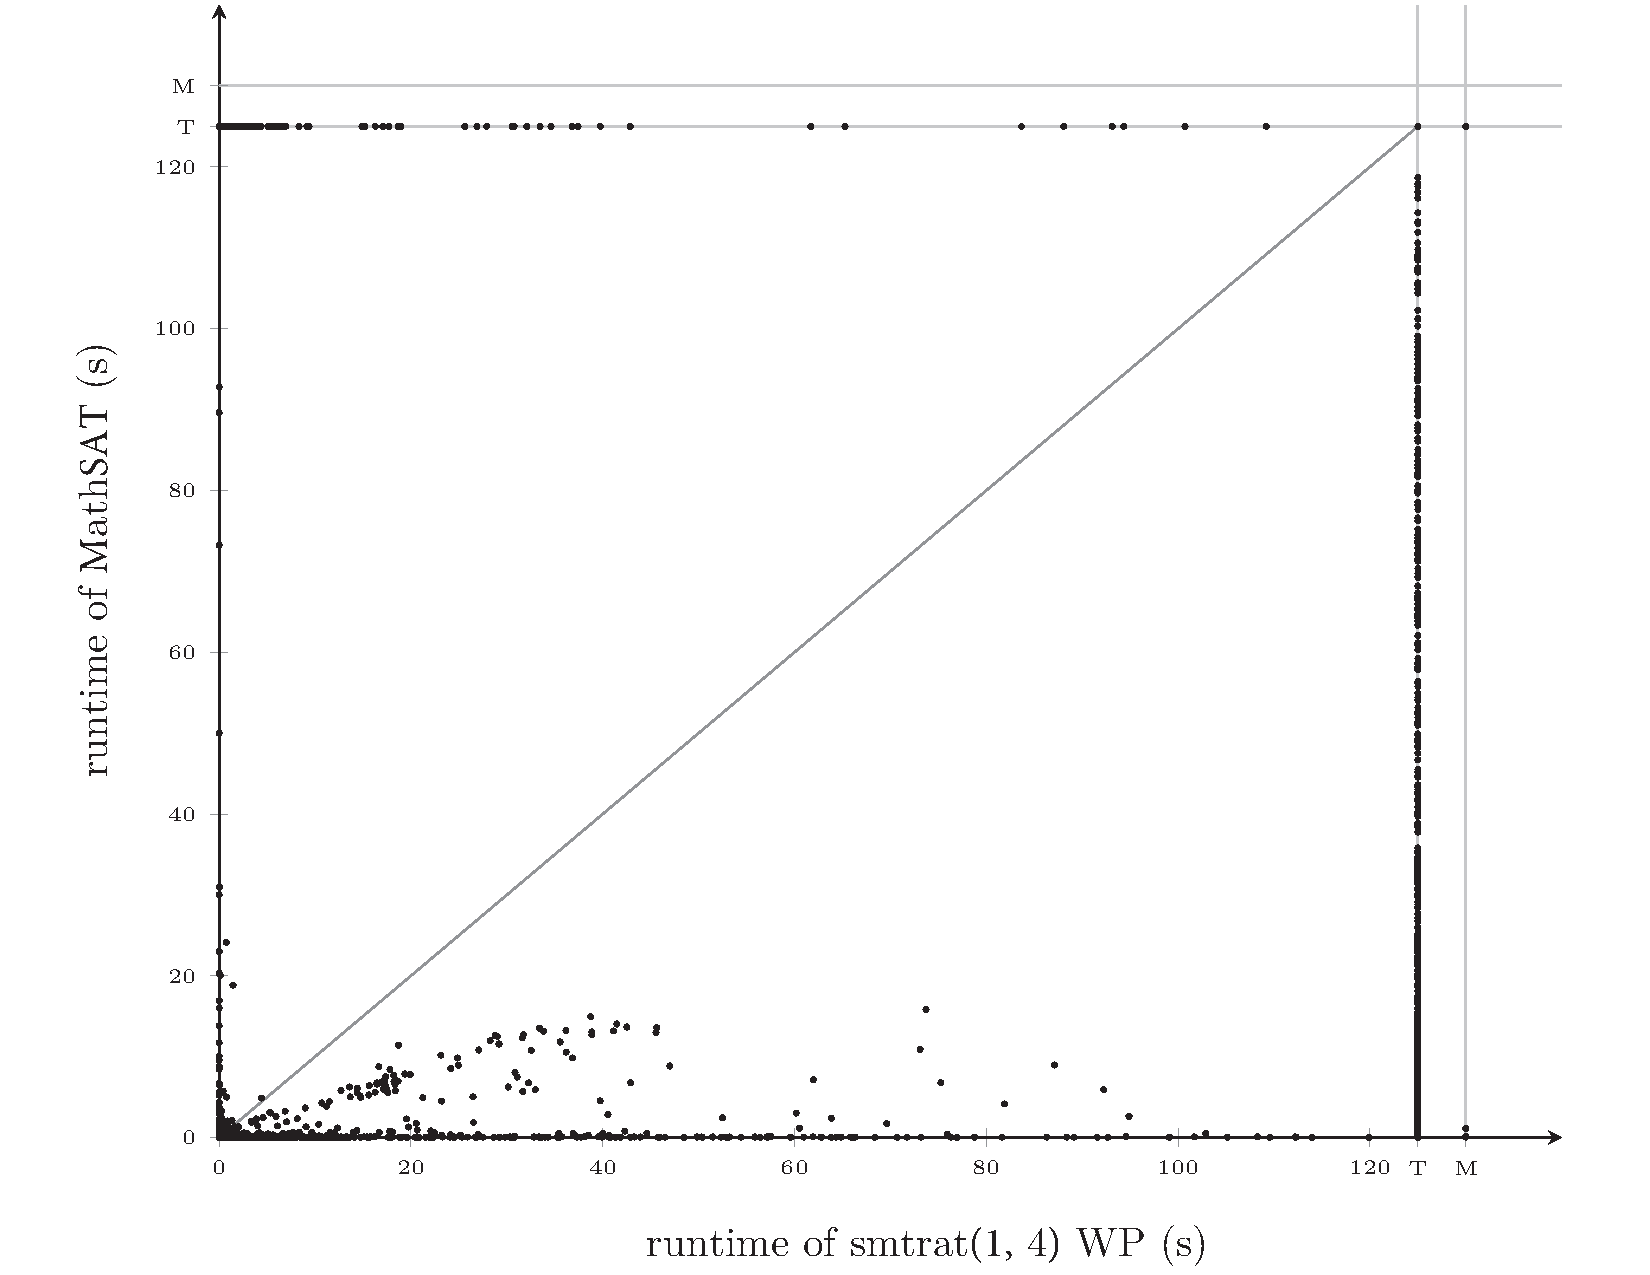
\includegraphics[width=.75\linewidth]{../figures/scatter-smtrat_4_preprocessing-mathsat-slide.pdf}
\end{figure}
\end{frame}

\section{Experimental Results}
\begin{frame}{Experimental Results}
\begin{figure}[!ht]
    \centering
    \caption{Scatter plot for smtrat(1, 4) WP and Z3}
    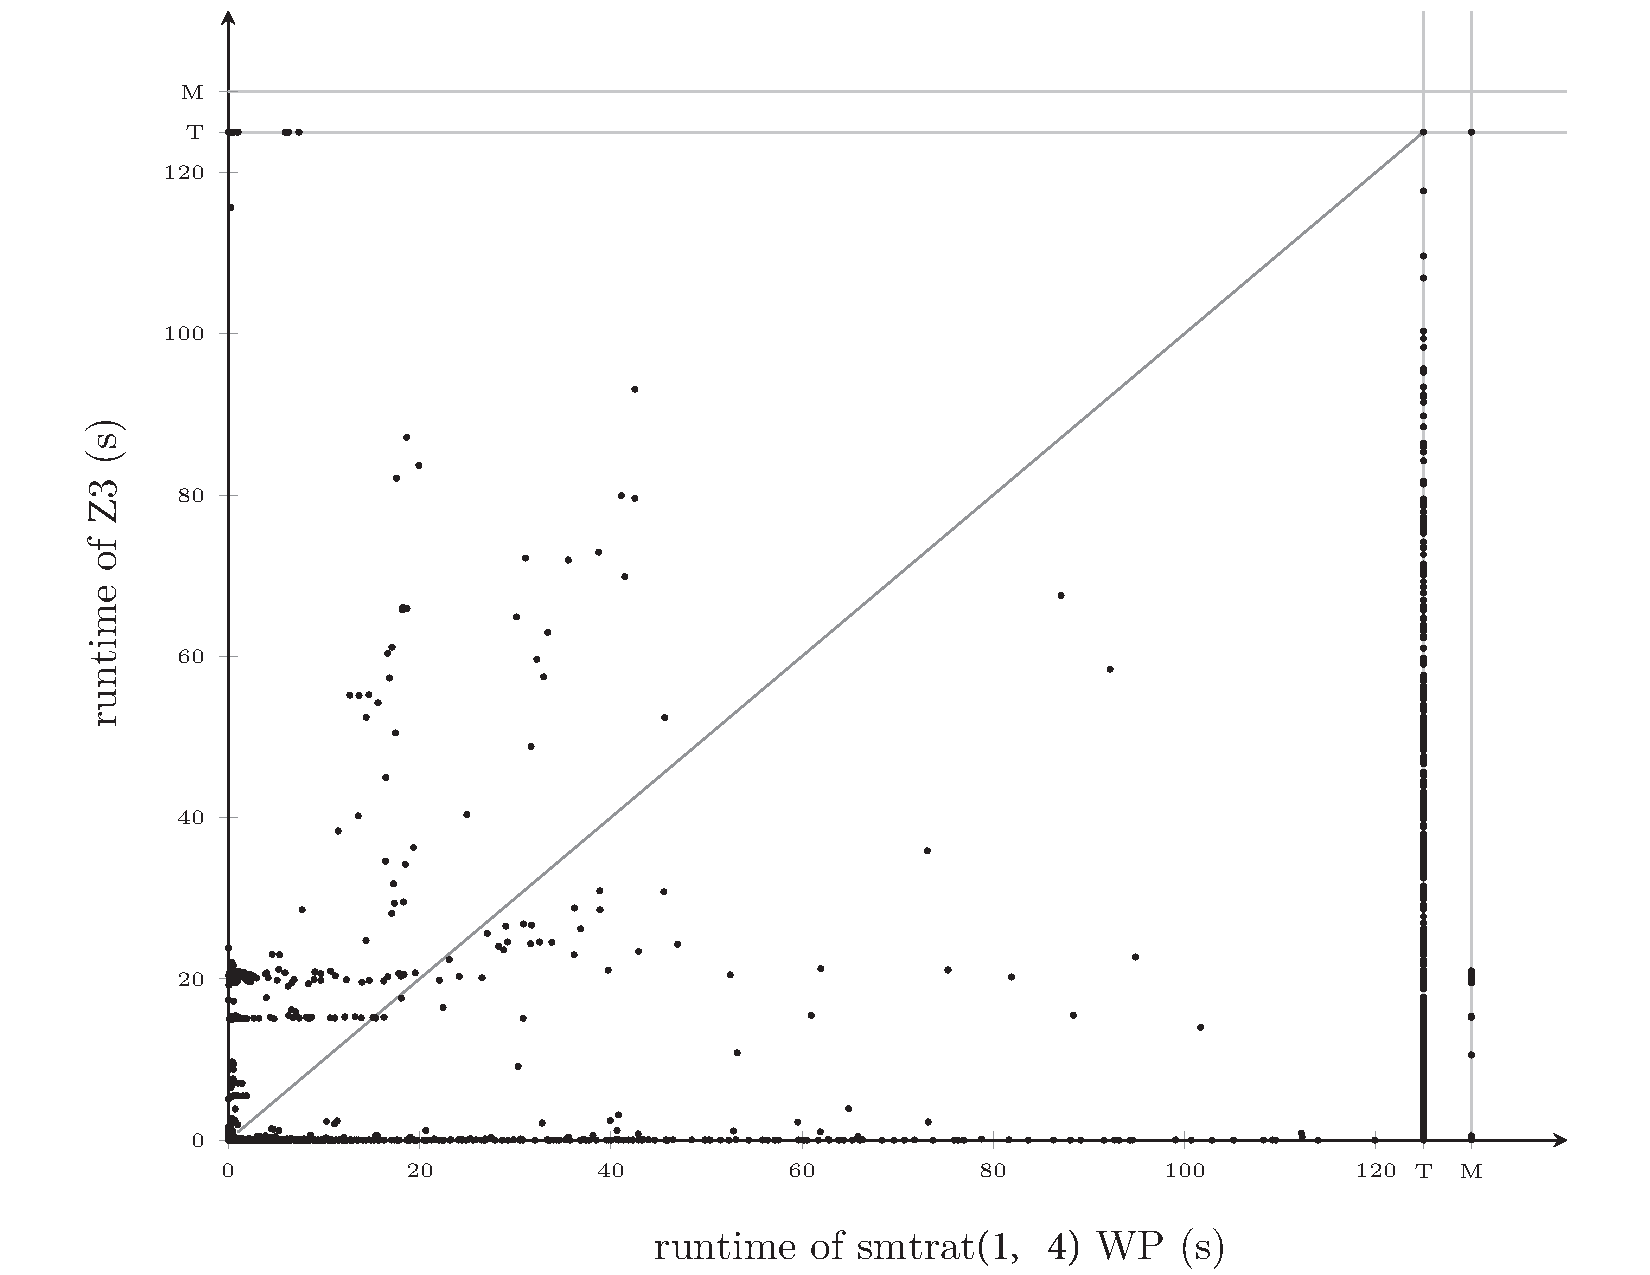
\includegraphics[width=.75\linewidth]{../figures/scatter-smtrat_4_preprocessing-z3-slide.pdf}
\end{figure}
\end{frame}

\section{Experimental Results}
\begin{frame}{Experimental Results}
\textcolor{blue}{\textbf{Additional SMT-RAT solvers: }smtrat(1, 8), smtrat(1, 9), smtrat(1, 10) and smtrat(1, 11).}
\begin{figure}[!ht]
    \centering
    \caption{Summary of smrat4, other additional smtrat solvers, mathsat and z3}
    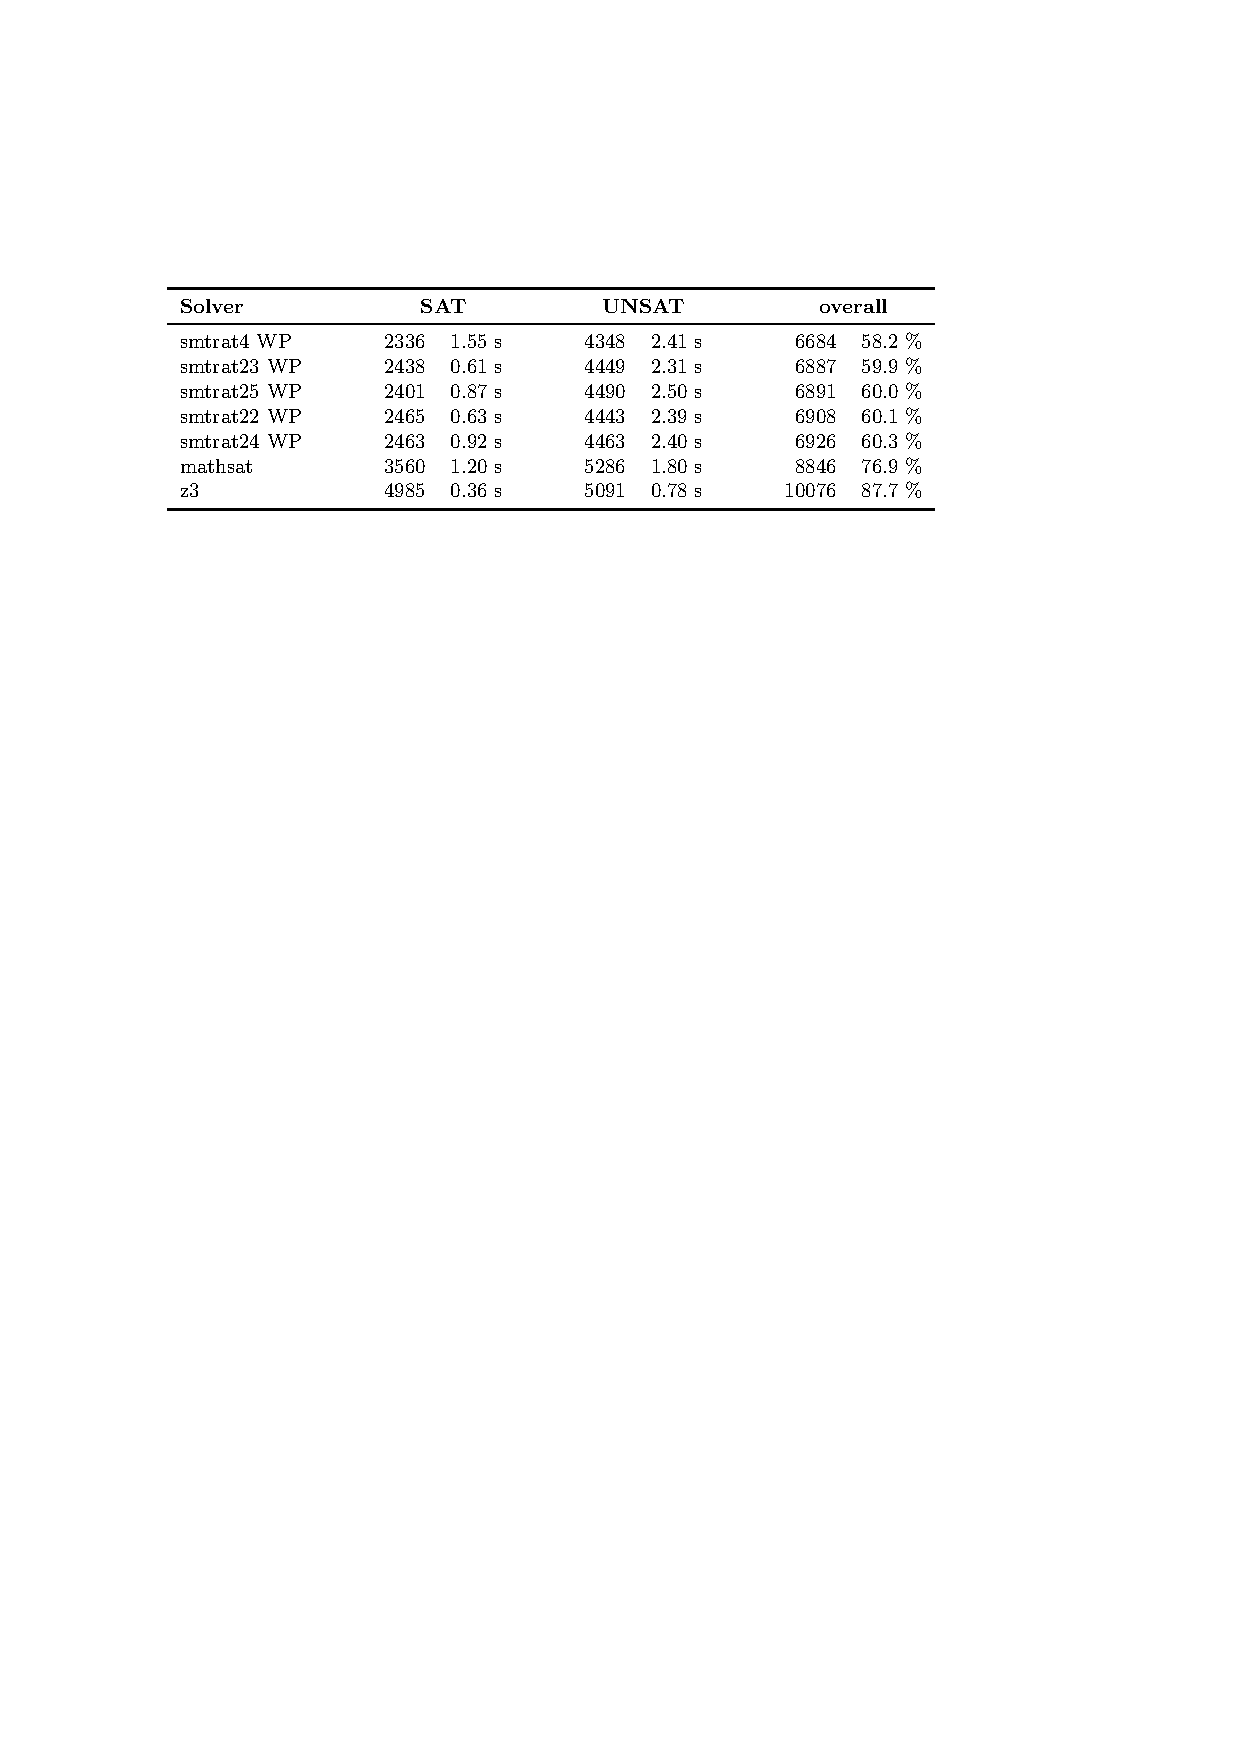
\includegraphics[width=1\linewidth]{../figures/summarySolvers.pdf}
\end{figure}
\end{frame}

\section{Future Work}
\begin{frame}{Future Work}
    \begin{itemize}
        \item \textcolor<1>{blue}{Currently: ICP excludes boxes.}\newline
        
        \textcolor<1>{red}{Future: exclude regions different shapes.}
        \bigskip
        \bigskip
        \item \textcolor<2>{blue}{Currently: extend the abstract model by guessing assignments.}\newline
        
        \textcolor<2>{red}{Future: repair the abstract model.}
    \end{itemize} 
\end{frame}

\section{Conclusion}
\begin{frame}{Conclusion}
    \begin{itemize}
        \item \textcolor<1>{blue}{Integrated this method as a module in SMT-RAT.}
        \bigskip
        \item \textcolor<1>{blue}{The module is a prototype.}
        \bigskip
        \item \textcolor<1>{blue}{Scopes available to enhance the performance.}
    \end{itemize}
\end{frame}
\end{document}

